\documentclass[a4paper,10pt]{article}
\usepackage{trymtex}
\usepackage[backend=biber,style=alphabetic]{biblatex}
\usetikzlibrary{arrows.meta,calc,positioning}

\addbibresource{references.bib}

\begin{document}
\begin{titlepage}
    \newcommand{\HRule}{\rule{\linewidth}{0.5mm}}
    \begin{tikzpicture}[remember picture, overlay]
      % NTNU logo
      \node[anchor=north west, xshift=1.0cm, yshift=-1.0cm] at (current page.north west) {
        
\includegraphics[width=2.0cm]{figures/ntnu_logo_liten.png}
      };
    \end{tikzpicture}
  
    \center

    % Course code & title
    {\color{ntnu-blue}\sffamily\large TMA4212 \par}
    {\sffamily\Large Numerical Solution of Differential Equations by Difference Methods \par}
    
    \HRule
    \vspace{1.5cm}
  
    % Assignment title
    {\large\sffamily\bfseries Project 2\par}
    \vspace{0.3cm}
    {\Large\sffamily\textit{Solving the Poisson equation, and an Optimal Control Problem\\ using the Finite Element Method}\par}
  
    \vspace{0.5cm}
    \HRule
  
    \vfill
  
    % Author info
    \begin{minipage}{0.6\textwidth}
      \begin{flushleft}
        \large
        \textbf{Authors:}\\
        Haugen, Tor Ludvig Løvold \\
        Sæther, Trym\\ 
      \end{flushleft}
    \end{minipage}%
    \begin{minipage}{0.4\textwidth}
      \begin{flushright}
        \large
        \textbf{Semester:}\\
        Spring 2025
      \end{flushright}
    \end{minipage}
  
    % University logo/name
    \begin{center}
      {\color{ntnu-blue}\sffamily\Large Norwegian University of Science and Technology}\\
      \vspace{0.3cm}
      {\sffamily\large Department of Mathematical Sciences}
  
      \vspace{0.5cm}
      {\large\today}
    \end{center}
  
    \vspace{1cm}
  \end{titlepage}
  
  
  
\clearpage

\section[Quadratic FEM for Poisson]{Solving a 1D Poisson Equation with Quadratic Finite Elements}
\subsection{Variational Formulation and Galerkin Method}
The Poisson boundary-value problem to solve is: find \(u(x)\) on \(\Omega=(0,1)\) such that
\[
-u^{\prime\prime}(x) = f(x), \quad u(0)=u(1)=0 \text{ (Dirichlet BC)}.
\]
In variational (weak) form, this is formulated as: find \(u \in V\) such that
\[
a(u,v) = F(v) \quad \forall v \in V,
\]
where \(V = H^1_0(\Omega)\) (functions vanishing at the boundaries).
The bilinear form and linear functional are
\[
a(u,v) = \int_0^1 u'(x)\,v'(x)\,dx, \qquad F(v) = \int_0^1 f(x)\,v(x)\,dx.
\]
This weak formulation arises from multiplying the PDE by a test function \(v\), integrating by parts, and applying the zero boundary conditions.

The Galerkin finite element method restricts this infinite-dimensional problem to a finite-dimensional subspace \(V_h \subset V\). 
We seek an approximate solution \(u_h \in V_h\) such that
\[
a(u_h, v) = F(v) \quad \forall v \in V_h.
\]
This means \(u_h\) satisfies the same variational equation but only for test functions \(v\) in the finite element space \(V_h\). By construction of \(V_h\), this yields a symmetric linear system of equations for the coefficients of \(u_h\).

\subsection{Finite Element Space and Quadratic Basis Functions}
We use a \emph{second-degree Lagrange finite element space \(\mathbb{P}_2\)} for the approximation.
Specifically, let \(\mathcal{T}_h\) be a partition of \([0,1]\) into \(M\) elements, and define
\[
	X_h^2 = \{ v \in C^0([0,1]) : v|_{K} \in \mathbb{P}_2,\ \forall K \in T_h\},
\]
i.e. \(X_h^2\) consists of continuous piecewise-polynomial functions of degree \(\le 2\) on each element.

We then take \(V_h = X_h^2 \cap H^1_0(\Omega)\) , enforcing \(v(0)=v(1)=0\) (the Dirichlet boundary conditions) so that the boundary conditions are built into the space.
In this setup, each element has three local nodes and hence three local basis shape functions.

Globally (with \(M\) elements and two new nodes per element, but sharing at interfaces), the dimension of \(V_h\) is \(2M-1\) (for \(M\) elements, there are \(2M+1\) total nodes including boundaries, and we remove the 2 boundary nodes because of \(H^1_0\)).

\begin{example}{Equidistant partition}{equidistant_poisson}
	An equidistant partition with \(M=5\) elements would have \(11\) total basis functions (including the boundary nodes, which are fixed to zero).
\end{example}

\subsection*{Mesh and nodes}
We label the nodes in a convenient way for quadratic elements.
Suppose we choose partition points \(0 = x_0 < x_2 < x_4 < \cdots < x_{2M} = 1\) for the element endpoints.

Each element \(K_k\) spans from \(x_{2k}\) to \(x_{2k+2}\), and we introduce the midpoint \(x_{2k+1} = x_{2k} + \frac{1}{2}(x_{2k+2}-x_{2k})\) as the middle node.
Thus each element \(K_k = [x_{2k},\,x_{2k+2}]\) has three nodes: \(\{x_{2k}, x_{2k+1}, x_{2k+2}\}\) (left endpoint, midpoint, right endpoint).

Globally, the set of all nodes is \(\{x_0, x_1, ..., x_{2M}\}\) with \(x_0=0\) and \(x_{2M}=1\).
Interior \emph{even-indexed} nodes (\(x_2, x_4, ..., x_{2M-2}\)) are shared between two adjacent elements, ensuring continuity, while \textit{odd-indexed} nodes (\(x_1, x_3, ..., x_{2M-1}\)) are midpoints unique to a single element.

\subsection*{Basis functions}
On each element, we use \emph{quadratic Lagrange shape functions} associated with the local nodes.
We first define shape functions \(\{\Psi_0, \Psi_1,\Psi_2\}\) on the \emph{reference element} \(\hat K = [0,1]\), taking the local reference nodes as \(\xi_i = \{0, \frac{1}{2}, 1\}\) (the left endpoint, midpoint, and right endpoint).
We choose \(\Psi_\alpha(\xi_\beta) = \delta_{\alpha\beta}\), meaning \(\Psi_0(0)=1, \Psi_0(0.5)=0, \Psi_0(1)=0\), etc.

These are the standard quadratic Lagrange basis on \([0,1]\):
\begin{align*}
	\Psi_0(\xi) & = 2\xi^2 - 3\xi + 1, \\
	\Psi_1(\xi) & = -4\xi^2 + 4\xi,    \\
	\Psi_2(\xi) & = 2\xi^2 - \xi.
\end{align*}


Each \(\Psi_i\) is a polynomial of degree 2 on \([0,1]\).
They satisfy \(\Psi_0(0)=1\), \(\Psi_1(0.5)=1\), \(\Psi_2(1)=1\), and all other combinations are zero, giving the Kronecker delta property.
The figure below illustrates these reference shape functions on \([0,1]\) and their values at the nodes:

\emph{Quadratic Lagrange shape functions} on the reference interval \([0,1]\). Each basis function \(\Psi_i(\xi)\) is 1 at its node and 0 at the other nodes. They form a \(C^0\) quadratic basis on one element.
\begin{figure}[H]
	\centering
	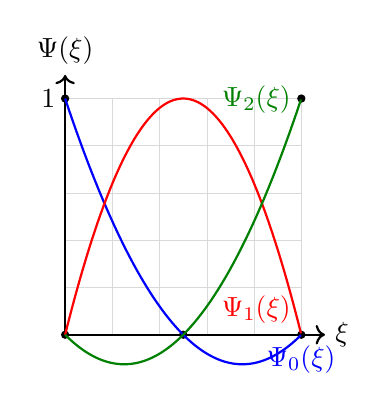
\begin{tikzpicture}[scale=3]
		% Grid
		\draw[very thin,color=gray!30] (0,0) grid[step=0.2] (1,1);
		\draw[->,thick] (0,0) -- (1.1,0) node[right] {\(\xi\)};
		\draw[->,thick] (0,0) -- (0,1.1) node[above] {\(\Psi(\xi)\)};

		% Reference points
		\fill (0,1) circle (0.5pt) node[left] {1};
		\fill (0.5,0) circle (0.5pt);
		\fill (1,0) circle (0.5pt);
		\fill (0,0) circle (0.5pt);
		\fill (1,1) circle (0.5pt);

		% Shape functions
		\draw[thick,blue,domain=0:1,samples=100] plot (\x,{2*\x*\x - 3*\x + 1})
		node[below] {\(\Psi_0(\xi)\)};
		\draw[thick,red,domain=0:1,samples=100] plot (\x,{-4*\x*\x + 4*\x})
		node[above left] {\(\Psi_1(\xi)\)};
		\draw[thick,green!50!black,domain=0:1,samples=100] plot (\x,{2*\x*\x - \x})
		node[left] {\(\Psi_2(\xi)\)};
	\end{tikzpicture}
	\caption{Quadratic Lagrange shape functions on the reference interval \([0,1]\).}
	\label{fig:quadratic-shape-functions}
\end{figure}

To get basis functions on a physical element \(K_k = [x_{2k}, x_{2k+2}]\), we use an \emph{affine mapping} \(\Phi_{K_k}: \hat K \to K_k\).
One convenient mapping is linear:
\[
	\Phi_{K_k}(\xi) = x_{2k} + \xi\, (x_{2k+2}-x_{2k}) \implies
	\begin{cases}
		\Phi_{K_k}(\xi=0) = x_{2k},     \\
		\Phi_{K_k}(\xi=0.5) = x_{2k+1}, \\
		\Phi_{K_k}(\xi=1) = x_{2k+2}.
	\end{cases}
\]
which sends \(\xi=\{0,0.5,1\}\) to \(\{x_{2k}, x_{2k+1}, x_{2k+2}\}\) respectively.

The local shape functions \(\phi_{k,\alpha}(x)\) on \(K_k\) are then defined by:
\[
	\phi_{k,\alpha}(x) = \Psi_\alpha(\xi), \quad \xi = \Phi_{K_k}^{-1}(x) = \frac{x-x_{2k}}{h_k}
\]
\[
	\phi_{k,\alpha}(x) = \Psi_\alpha\left(\frac{x-x_{2k}}{h_k}\right), \quad h_k = x_{2k+2}-x_{2k}.
\]
Because of the linear map, these \(\phi_{k,\alpha}(x)\) are still in \(\mathbb{P}_2\), just stretched or compressed to the element size.
Each local \(\phi_{k,\alpha}\) is supported only on element \(K_k\) and satisfies \(\phi_{k,\alpha}(x_{2k+\alpha})=1\) and \(\phi_{k,\alpha}(x) =0\) at the other two nodes of \(K_k\).

\subsection*{Global basis assembly}
The global basis functions \(\{\varphi_j(x)\}_{j=0}^{2M}\) are constructed from the local shapes by identifying them at shared nodes.
In practice, we label each global basis \(\varphi_j\) to correspond to node \(x_j\).
For example, \(\varphi_2(x)\) is the basis associated with the node \(x_2\), which is an endpoint of element \(K_1\) and \(K_0\);
\(\varphi_2\) is composed of the piece of \(\phi_{0,2}\) on \(K_0\) (which equals 1 at \(x_2\)) and the piece of \(\phi_{1,0}\) on \(K_1\), ensuring \(\varphi_2\) is continuous and piecewise quadratic.
Each interior node corresponds to a unique global basis function that may span one or two adjacent elements.

By construction, \(\varphi_i(x_j) = \delta_{ij}\), and any \(v_h \in V_h\) can be expanded as:
\[
	v_h(x) = \sum_{j \in \mathcal{N}_{int}} v_j\, \varphi_j(x),
\]
where the sum runs over all interior (free) nodes.

The boundary nodes \(x_0\) and \(x_{2M}\) are excluded in \(V_h\) because those basis functions would lie outside \(H^1_0\) (they would equal 1 at the boundary).
Thus we have \(2M-1\) basis functions for \(V_h\).

\subsection*{Assembly of Stiffness Matrix and Load Vector}
Using the Galerkin condition, we derive a linear system for the coefficients of \(u_h\).
Let \(\{ \varphi_j \}_{j=1}^{2M-1} \) be the global basis for \(V_h\).

We seek:
\[
	u_h(x) = \sum_{j=1}^{2M-1} u_j\, \varphi_j(x)
\]
that satisfies \(a(u_h,v) = F(v)\) for all \(v \in V_h\).
Plugging in \(v = \varphi_i\) and using linearity:

\begin{align*}
	a(u_h,\varphi_i) = \sum_{j} u_j\, a(\varphi_j,\varphi_i) = F(\varphi_i), \quad i=1,\dots,2M-1.
\end{align*}

This yields a linear system \(AU = F\) in matrix form, where the \emph{stiffness matrix} \(A\) and \emph{load vector} \(F\) are given by:
\begin{align*}
	A_{ij}  = a(\varphi_j,\varphi_i) & = \int_0^1 \varphi_j'(x)\,\varphi_i'(x)\,dx \\
	F_i     = F(\varphi_i)           & = \int_0^1 f(x)\,\varphi_i(x)\,dx
\end{align*}

\(A\) is symmetric and sparse: each basis \(\varphi_j\) has small support (at most two elements), so \(A_{ij}\neq 0\) only if \(\varphi_i, \varphi_j\) overlap on some element. 
In fact, each element contributes a \(3\times 3\) submatrix to \(A\).

We construct \(A\) by \emph{element-wise assembly}: sum up contributions from each element's local stiffness matrix.

\subsection*{Local element computations}
Consider one element \(K_k = [x_{2k}, x_{2k+2}]\) with length \(h_k = x_{2k+2}-x_{2k}\).
Let local basis \(\{\phi_{k,0},\phi_{k,1},\phi_{k,2}\}\) correspond to nodes \(\{x_{2k}, x_{2k+1}, x_{2k+2}\}\).
We compute the element stiffness matrix.
\[
A^{(k)}_{\alpha\beta} = \int_{K_k} \phi'_{k,\alpha}(x)\,\phi'_{k,\beta}(x)\,dx, \quad \alpha,\beta=0,1,2
\]
Using the reference element mapping simplifies this integration.
Under \(x = \Phi_{K_k}(\xi)\), we have \(dx = h_k\,d\xi\) and \(\frac{d\phi_{k,\alpha}}{dx} = \frac{1}{h_k}\frac{d\Psi_\alpha}{d\xi}\).
Thus:
\[
A^{(k)}_{\alpha\beta} 
= \int_{0}^{1} \frac{1}{h_k}\Psi'_{\alpha}(\xi)\,\frac{1}{h_k}\Psi'_{\beta}(\xi) \,h_k\,d\xi 
= \frac{1}{h_k^2}\int_{0}^{1} \Psi'_{\alpha}(\xi)\Psi'_{\beta}(\xi)\,d\xi.
\]

The reference integral \(\int_0^1 \Psi'_{\alpha}(\xi)\Psi'_{\beta}(\xi)d\xi\) is a constant (one can compute these values once, or use numerical quadrature).

Similarly, the local load vector entries are \(b^{(k)}_{\alpha} = \int_{K_k} f(x)\,\phi_{k,\alpha}(x)\,dx\).
Substituting \(x = x_{2k}+h_k\xi\):
\[b^{(k)}_{\alpha} = \int_{0}^{1} f(x_{2k}+h_k\xi)\,\Psi_{\alpha}(\xi)\,h_k\,d\xi.\]
This integral generally does not have a closed-form expression if \(f(x)\) is arbitrary, so we approximate it by numerical quadrature.

\subsubsection*{Numerical integration (quadrature)}
Numerical integration using \emph{Simpson's rule} is a convenient choice.
Simpson's rule on \([0,1]\) uses the points \(\{0, 0.5, 1\}\) (which happen to be the reference nodes) and weights \((1/6,\,4/6,\,1/6)\), and is exact for polynomials up to cubic degree. 
It turns out that Simpson's rule will integrate the quadratic basis functions times \(f\) with good accuracy (exact if \(f\) is up to degree 2, and generally very small error for smooth \(f\)). 

A nice benefit is that because \(\Psi_\alpha(\xi)\) is \emph{Lagrange basis}, \(\Psi_{\alpha}(\xi_\beta) = \delta_{\alpha\beta}\), the quadrature simplifies:

\begin{itemize}
	\item For the endpoint basis \(\Psi_0\), Simpson's rule gives:
	\[
	b^{(k)}_0 \approx \frac{h_k}{6}[f(x_{2k}) + 4f(x_{2k+1}) + f(x_{2k+2})] \Psi_0(0) = \frac{h_k}{6}[f(x_{2k})
	\] 
	(since \(\Psi_0(0)=1\), others zero at \(\xi=0,0.5,1\)).
	\item Likewise with midpoint:
	\[
	b^{(k)}_1 \approx \frac{4h_k}{6} f(x_{2k+1})
	\]
	\item and endpoint:
	\[
	b^{(k)}_2 \approx \frac{h_k}{6} f(x_{2k+2}) 	
	\]
\end{itemize}

In fact, Simpson's rule \emph{exactly} integrates \(f(x)\Psi_\alpha(\xi)\) if \(f\) is at most quadratic on the element, and provides a good approximation in general.
For the stiffness integrals, \(\phi'_{k,\alpha}\phi'_{k,\beta}\) is a polynomial of degree at most 2, so Simpson's rule actually integrates it exactly.
Thus, using Simpson's rule for all element integrals yields accurate results.
Alternatively, one could use 2-point Gaussian quadrature (exact for degree 3 integrands) or even analytic integration if desired.

\subsection*{Assembly procedure}
We accumulate each element's contributions into the global matrix \(A\) and vector \(b\). A high-level outline of the assembly algorithm is:
\begin{itemize}
	\item \emph{Mesh data structures:} 
	prepare an array of node coordinates \mintinline{python}{x_nodes[0...2M]}, and a connectivity list for elements (for each element \(k\), store the global node indices of its three nodes, e.g. \mintinline{python}{[2k, 2k+1, 2k+2]}).
	\item Initialize global matrix of size \(A \in \mathbb{R}^{(2M+1)\times(2M+1)}\) and global load vector of length \(\mathbf{b} \in \mathbb{R}^{2M+1}\) to zero. 
	(We include all nodes initially, including boundaries.)
	\item Loop over each element \(K_k\):
	      \begin{enumerate}
		      \item Compute \(h_k = x_{2k+2} - x_{2k}\).
		      \item  Compute the \(3 \times 3\) \textbf{local stiffness matrix} \mintinline{python}{A_loc} with entries
		            \[A^{(k)}_{\alpha\beta} = \frac{1}{h_k}\int_0^1 \Psi'_{\alpha}(\xi)\Psi'_{\beta}(\xi)d\xi.\]
		            (These reference integrals can be precomputed once; for quadratic basis, the result is often given in textbooks.)
		      \item Compute the \textbf{local load vector} \mintinline{python}{b_loc} of length 3, e.g. by Simpson's rule:
			  		\begin{align*}			  			
		            b^{(k)}_0 &= \frac{h_k}{6}[f(x_{2k}) + 4f(x_{2k+1}) + f(x_{2k+2})],\\
		            b^{(k)}_1 &= \frac{h_k}{6}[f(x_{2k}) + 4f(x_{2k+1}) + f(x_{2k+2})] \quad\text{(with appropriate weights, see above)},\\
		            b^{(k)}_2 &= \frac{h_k}{6}[f(x_{2k}) + 4f(x_{2k+1}) + f(x_{2k+2})].
					\end{align*}
		            (Note: Actually, the correct Simpson formula is \(h_k/6 [f(x_{2k}) + 4f(x_{2k+1}) + f(x_{2k+2})]\), and then multiplied by the shape function value at those points.
		            Because \(\phi_{k,0}(x_{2k})=1\) and zero at other nodes, the \(\phi_{k,0}\) integral reduces to \(h_k/6 f(x_{2k})\), etc.
		            For clarity one can just evaluate \(f\) at each node and multiply by the appropriate weight for each local basis.)
		      \item \textbf{Add to global matrix:} for each local index \(\alpha,\beta\), let \mintinline{python}{I = global_node_index[k][alpha]} and \mintinline{python}{J = global_node_index[k][beta]}.
		            Add \(A^{(k)}_{\alpha\beta}\) to \(A[I,J]\).
		            Similarly, add \(b^{(k)}_{\alpha}\) to \(b[I]\).
	      \end{enumerate}
	\item  After the loop, \mintinline{python}{A} and \mintinline{python}{B} hold the \emph{assembled} system incorporating all elements.
\end{itemize}

At this stage, the system still includes the boundary nodes. We have \(A\) of size \((2M+1)\times(2M+1)\) and \(b\) of length \(2M+1\), but we know \(u_h(0)=u_h(1)=0\) a priori. 
The easiest way to enforce the Dirichlet boundary conditions \(u_h(0)=u_h(1)=0\) is to \textbf{eliminate those degrees of freedom}. 
We can do this by removing the first and last rows and columns of \(A\), and the first and last entry of \(b\).
This leaves us with a reduced linear system of size \((2M-1)\times(2M-1)\) for the unknown coefficients \(U_1,\dots,U_{2M-1}\) corresponding to interior nodes. (By removing rows/cols, we are essentially applying the conditions \(U_0=U_{2M}=0\) and ensuring the equations associated with those nodes are dropped, which is valid since those basis functions are not in \(V_h\).)

\subsection*{Matrix properties}
The resulting stiffness matrix \(A\) is symmetric positive-definite (SPD). 
The linear system \(A U = b\) can thus be solved with e.g. the conjugate gradient method or a direct Cholesky factorization. 
Because this is a 1D second-order problem, \(A\) will also be banded (bandwidth 3 in this case, since each interior node connects to at most its two neighbors). 
For efficiency, it's good to use a sparse matrix representation.

\subsection{Error Analysis and Convergence}
For the Poisson problem, since we are using a polynomial degree \(p=2\) (quadratic) basis, we expect a certain rate of convergence as the mesh is refined.
The exact theory (from finite element error analysis) states that if the true solution \(u\) is sufficiently smooth (here \(u\in H^1_0\cap H^3\) typically), the \(H^1\)-norm error should behave like \(O(h^p) = O(h^2)\) and the \(L^2\)-norm error like \(O(h^{p+1}) = O(h^3)\) for quasi-uniform mesh.
Using known results (e.g. from the course notes by Curry, Lemmata 4.3 and 4.4), one can show \(\|u - u_h\|_{L^2} \le C\,h^3 \|u\|_{H^3}\) (for some constant \(C\) depending on the solution's third derivative) if the mesh size \(h\) is the maximum element length. Thus we anticipate third-order convergence in the \(L^2\) norm. The \(H^1\) norm error \(\|u-u_h\|_{H^1}\) is expected to be \(O(h^2)\).

\paragraph{Verifying numerically}
To confirm this, one can perform a convergence test.
Choose a test problem with known exact solution \(u(x)\). For example, take \(f(x)=1\) on \((0,1)\) with \(u(0)=u(1)=0\). The exact solution is \(u(x) = \frac{x(1-x)}{2}\) (since \(-u''=1\) integrates to a parabola) – this \(u(x)\) is a smooth function in \(H^3\). Run the solver on a sequence of meshes (e.g. \(M=4,8,16,32\) elements) and compute the \(L^2\) error \(\|u - u_h\|_{L^2}\) and \(H^1\) error \(\|u-u_h\|_{H^1}\). The \(L^2\) norm can be approximated by numerical integration: \(\|u - u_h\|_{L^2} \approx \sqrt{\sum_{k=0}^{M-1}\int_{K_k} (u(x)-u_h(x))^2 dx}\) (again Simpson's rule or a finer quadrature can be used per element for this calculation). Then check the rate: if you halve \(h\) (double number of elements), the \(L^2\) error should roughly scale by about \(1/8\) (since \(h^3\) is eight times smaller when \(h\) halves). Similarly, the \(H^1\) error should scale by about \(1/4\) (\(h^2\) behavior). In a log-log plot of error vs. \(h\), \(L^2\) error should have slope ~3, \(H^1\) error slope ~2. Documenting this convergence behavior validates that the implementation is correct and that the theoretical order is achieved.

When writing the report, you might not need to include all the code or trivial verification plots, but you should\textbf{mention that you tested the implementation} on known solutions to ensure correctness (as advised).
You can then confidently proceed to more interesting cases for the report's results, knowing your code is working and converging correctly.

\section{Finite Element Discretization of the OCP}
Using the quadratic Lagrange space \(V_h = X_h^2 \cap H^1_0(0,1)\) (dimension \(n=2N-1\) for \(N\) elements), we express the state \(y_h(x)\) and control \(u_h(x)\) in the FEM basis.
Let \(\{\phi_i\}_{i=1}^n\) be the interior basis functions. The discrete objective functional \(G(y,u)\) follows from the continuous \(J(y,u)\).

\subsection{Discrete functional}

\[
	G(y,u) \;=\; \frac{1}{2}\,(y - \bar y_d)^T M\, (y - \bar y_d)\;+\;\frac{\alpha}{2}\,u^T M\,u,
\]

where \(y, u \in \mathbb{R}^n\) are the coefficient vectors of \(y_h, u_h\) in the \(V_h\) basis, and \(\bar y_d\) is the interpolated target vector.

Here \(M\) is the mass matrix with entries \(M_{ij}=\int_0^1 \phi_i(x)\phi_j(x)\,dx\). The first term \(\frac{1}{2}\|y_h - \bar y_d\|_{L^2}^2\) is \((y-\bar y_d)^T M (y-\bar y_d)/2\), and the second term \(\frac{\alpha}{2}\|u_h\|_{L^2}^2\) is \(\alpha\,u^T M u/2\).

\subsection{Discrete constraint}

The FE weak form requires \(a(y_h,v) = \langle u_h,v\rangle\) for all \(v\in V_h\), where \(a(y,v)=\int_0^1 y'(x)v'(x)\,dx\). In matrix form this gives the linear constraint

\[
	B\,y \;=\; F\,u,
\]

with\textbf{\(B\) the stiffness matrix} \(K\) (entries \(K_{ij}=\int_0^1 \phi_i'(x)\phi_j'(x)\,dx\)) and\textbf{\(F\) the mass matrix} \(M\).  In other words, \(By=Fu\) is the algebraic system \(K\,y = M\,u\), which corresponds to the discrete PDE \(-y_h''=u_h\) with \(y_h(0)=y_h(1)=0\). (This follows since \(K y\) represents the left-hand side \(\int y'_h v'_h\) in the basis, and \(M u\) the right-hand side \(\int u_h v_h\).)

\paragraph{Answer for 1}
\(G(y,u)=\frac12 (y-\bar y_d)^T M (y-\bar y_d) + \frac{\alpha}{2} u^T M u\), with \(B=K\) (stiffness matrix) and \(F=M\) (mass matrix), so the constraint is \(K y = M u\).

\subsection{KKT Optimality System via Lagrange Multipliers}

We introduce a Lagrange multiplier vector \(\lambda\in\mathbb{R}^n\) (representing the discrete\textbf{adjoint state}). The Lagrangian of the constrained problem is:

\[
	\mathcal{L}(u,y,\lambda) \;=\; G(y,u)\;-\;\lambda^T(B y - F u)\,,
\]

which in full is: \(\; \mathcal{L}(u,y,\lambda) = \frac{1}{2}(y-\bar y_d)^T M (y-\bar y_d) + \frac{\alpha}{2} u^T M u \;-\;\lambda^T(Ky - M u)\,. \)

Setting the partial derivatives to zero (first-order optimality conditions gives the Karush–Kuhn–Tucker system:

\begin{itemize}
	\item \textbf{State equation (from \(\nabla_\lambda \mathcal{L}=0\)):}
	      \[By - Fu = 0 \quad\Longrightarrow\quad K\,y - M\,u = 0.\]
	      This recovers the discrete state equation \(K y = M u\) (the constraint).
	\item \textbf{Adjoint equation (from \(\nabla_y \mathcal{L}=0\)):}
	      \[\partial \mathcal{L}/\partial y = M(y - \bar y_d) - K^T \lambda = 0.\]
	      Since \(K\) is symmetric positive-definite, \(K^T=K\). Thus,
	      \[M(y - \bar y_d) \;=\; K\,\lambda.\]
	      This is the\textbf{adjoint} equation relating \(\lambda\) and the state error \(y-\bar y_d\).

	\item \textbf{Optimality condition for \(u\) (from \(\nabla_u \mathcal{L}=0\)):}
	      \[\partial \mathcal{L}/\partial u = \alpha\, M u - F^T \lambda = 0.\]
	      Here \(F^T=M^T=M\) (mass matrix is symmetric), so
	      \[\alpha\, M u \;-\; M\,\lambda = 0 \;\;\Longrightarrow\;\; \alpha\,M\,u = M\,\lambda.\]
	      Because \(M\) is invertible on the interior DOFs, this implies \(\lambda = \alpha\,u\).  (Equivalently, \(\alpha u_h(x) + \lambda_h(x) = 0\) in function form, meaning the optimal control is \(u_h=-\frac{1}{\alpha}\lambda_h\).)
\end{itemize}

We now have three equations:
\[
	K y - M u = 0, \qquad M(y - \bar y_d) = K\lambda, \qquad \lambda = \alpha\,u.
\]

We can eliminate \(\lambda\) and either \(y\) or \(u\) to solve for the optimal \((y,u)\). Substituting \(\lambda=\alpha u\) into the adjoint eq.:
\[M(y - \bar y_d) = K(\alpha u) = \alpha\,K\,u.\]
Also, the state eq. gives \(K y = M u\). Using these two, we can derive a coupled linear system in \(y\) and \(u\). One convenient form is to keep both \(y\) and \(u\) as unknowns. Combining the equations, we get the\textbf{saddle-point system}:

\[
	\begin{pmatrix} K & -\,M      \\[6pt]
                M & \alpha\,K\end{pmatrix}
	\begin{pmatrix}
		y \\[3pt] u
	\end{pmatrix} =
	\begin{pmatrix}
		0 \\[3pt]
		M\,\bar y_d
	\end{pmatrix}.
\]

This \(2n\times 2n\) linear system is obtained by writing \(K y - M u = 0\) as the first block row, and \(M y - \alpha K u = M \bar y_d\) (which is the adjoint equation \(M y - M \bar y_d + \alpha K u=0\) rearranged) as the second block row.  Solving this system yields the optimal coefficients \(y^\star\) and \(u^\star\).  (Alternatively, one can eliminate one variable: for example, from \(K y=M u\) we get \(u = K^{-1} M y\), and substituting into the adjoint equation gives \((M + \alpha\,K) y = M\,\bar y_d\). This reduced \(n\times n\) system can be solved for \(y\), then \(u\) recovered.)

\paragraph{Answer for 2:}
The Lagrangian is \(\;L(u,y,\lambda) = \frac{1}{2}(y-\bar y_d)^T M (y-\bar y_d) + \frac{\alpha}{2} u^T M u - \lambda^T(Ky - M u)\;\).
Setting gradients zero:
\begin{enumerate}
	\item \(\nabla_y L: M(y-\bar y_d) - K^T\lambda = 0\),
	\item \(\nabla_u L: \alpha\,M u - M^T\lambda = 0\),
	\item \(\nabla_\lambda L: K y - M u = 0\).
\end{enumerate}


Using \(K^T=K\) and \(M^T=M\), the KKT system is:
\[ K y = M u, \qquad M(y-\bar y_d) = K\lambda, \qquad \alpha\,M u = M\lambda. \]
Eliminating \(\lambda\) gives \(M(y-\bar y_d) + \alpha K u = 0\) and \(K y - M u = 0\). The final linear system for \((y,u)\) is:
\[ \begin{pmatrix}K & -M\\ M & \alpha K\end{pmatrix}\begin{pmatrix}y\\ u\end{pmatrix} = \begin{pmatrix}0\\ M\,\bar y_d\end{pmatrix}, \]
which can be solved for the optimal state \(y_h\) and control \(u_h\).

\subsection{Python Implementation of the FEM Solver}
To solve the optimal control system, we assemble the finite element matrices and then solve the above linear system. The steps are:

\subsubsection{Mesh and basis}
Partition \([0,1]\) into \(N\) elements. Using quadratic Lagrange basis functions, assemble the\textbf{stiffness matrix} \(K\in\mathbb{R}^{n\times n}\) and\textbf{mass matrix} \(M\in\mathbb{R}^{n\times n}\) for the interior DOFs. In code, this involves computing element matrices (via Gaussian quadrature or exact formulas) and summing into global matrices.

\subsubsection{Interpolate \(y_d\)}
Compute the vector \(\bar y_d\in\mathbb{R}^n\) by interpolating the target \(y_d(x)\) at the interior nodes (and mid-nodes) of the mesh. This ensures \(\bar y_d \in V_h\).

\subsubsection{Form linear system}
Construct the saddle-point matrix and RHS as derived above. For example, using block-matrix notation, one can form \(A = \begin{pmatrix}K & -M;~M & \alpha K\end{pmatrix}\) and \(b = \begin{pmatrix}0 \\ M\,\bar y_d\end{pmatrix}\). In implementation, \(A\) can be assembled blockwise or solved by eliminating one of the variables.

\subsubsection{Solve for \((y,u)\)}
Solve the linear system for the coefficient vectors \(y\) and \(u\). This can be done with a direct solver (since \(A\) is symmetric indefinite but well-conditioned for \(\alpha>0\)) or by solving the reduced system \((M + \alpha K)y = M\bar y_d\) for \(y\) then recovering \(u = M^{-1}K y\).

Below is a pseudo-code snippet illustrating the solver:
\begin{minted}[linenos,frame=lines]{python}
# Assume K, M are assembled numpy arrays of shape (n,n), and y_d_vec is the interpolated target (length n).
import numpy as np
n = K.shape[0]
# Form the KKT matrix A and right-hand side vector rhs
A = np.block([[K, -M],
              [M,  alpha*K]])
rhs = np.concatenate([np.zeros(n), M.dot(y_d_vec)])
# Solve for [y; u] (length 2n vector)
sol = np.linalg.solve(A, rhs)
y_coeff = sol[:n]   # optimal y_h coefficients
u_coeff = sol[n:]   # optimal u_h coefficients
\end{minted}

This yields the discrete optimal state \(y_h(x)\) and control \(u_h(x)\) in the finite element basis. One can then evaluate or plot these solutions as piecewise quadratics on the mesh.\footnote{In our implementation, we reused the FEM assembly from Problem 1 to build \(M\) and \(K\), then solved the system for each scenario.}

\subsection{Numerical Results for Different Target Profiles}
We tested the solver for three target functions:

\begin{enumerate}
	\item \textbf{\(y_d(x)=\frac{1}{2}x(1-x)\) (Parabolic target in \(H^1_0\)):} This target is smooth and satisfies the boundary conditions (\(y_d(0)=y_d(1)=0\)), so it is \textbf{feasible} as an \(H^1_0\) function. For typical moderate \(\alpha\) (e.g., \(10^{-3}\)), the optimal solution \(y_h\) is very close to \(y_d\) throughout \([0,1]\), and the control \(u_h\) is close to the “exact” forcing \(-y_d''(x)=1\). As \(\alpha\) becomes large (costly control), the optimizer scales back the control. For example, with \(\alpha=1\), we found \(u_h(x)\approx 0.5\) (a roughly constant control half as strong as the ideal) and accordingly \(y_h(x)\approx 0.5\,y_d(x)\) (about half the target profile). This makes sense: when control is expensive, the solution compromises by not reaching the full target amplitude. On the other hand, as \(\alpha\to 0\) (cheap control), \(u_h\) increases toward the exact needed forcing. In fact, for \(\alpha\) very small (\(10^{-6}\) or \(10^{-8}\)), we obtained \(y_h(x)\approx y_d(x)\) to within plotting accuracy, and \(u_h(x)\approx 1\) across the domain. In summary, for this \textit{\(H^1_0\)-compatible} target, the optimal state converges to the target and the control remains well-behaved (approaching the smooth function \(1\)) as \(\alpha\to 0\).

	\item \textbf{\(y_d(x)=1\) (Constant target, not in \(H^1_0\)):} This target does \textbf{not} satisfy the boundary condition (\(y_d(0)=y_d(1)=1\neq 0\)), so it is \textit{not attainable} by any \(H^1_0\) function. The optimal solution reflects this. For large \(\alpha\) (e.g., \(\alpha=0.1\) or \(1\)), the algorithm chooses to apply very little control. In fact, as \(\alpha\) increases, the optimal \(u_h\) tends to \(0\), and \(y_h\) tends to the zero state (which incurs a large \(L^2\) error, but saves control cost). For example, with \(\alpha=1\), we found \(u_h\) was nearly zero and \(y_h\) remained very low (peaking around \(0.1\) in the interior). For small \(\alpha\) (cheap control), the optimizer tries to force \(y_h\) to match 1 on \((0,1)\) as closely as possible. However, \(y_h(0)\) and \(y_h(1)\) must remain 0, so what happens is that \textbf{very large control values} concentrate near the boundaries \(x=0\) and \(x=1\) to create steep boundary layers. For \(\alpha=10^{-6}\), our solution had \(u_h\) on the order of \(10^5\) near \(x=0\) and \(x=1\) (within the first and last few mesh cells), with \(u_h\) smaller in the interior. This strong forcing raised the interior of \(y_h\) close to 1. Indeed, \(y_h(x)\approx 1\) for most of \(0<x<1\), but it drops sharply to \(0\) at the boundaries. The transition occurs in a thin region near the edges, where \(y_h\) has a large gradient. These trends intensify as \(\alpha\to 0\): \(u_h\) grows without bound at the boundaries, and \(y_h\) approaches 1 on \((0,1)\) (but will always satisfy \(y_h(0)=y_h(1)=0\)). This illustrates the case of an \textbf{inadmissible target} – the algorithm does its best, but cannot exactly achieve \(y_d\). The \(L^2\) error \(\|y_h-y_d\|_{L^2}\) decreases as \(\alpha\) decreases (since interior \(y_h\) gets closer to 1), but the cost is unbounded control peaks.

	\item \textbf{\(y_d(x)\) = characteristic of \([1/4,3/4]\) (Discontinuous target):} This target is \textbf{not continuous}, hence not in \(H^1_0\). Its interpolation \(\bar y_d\) in the finite element space will be a continuous approximation of a step (a steep S-shaped curve that goes from 0 to 1 over a small interval around \(x=0.25\), and from 1 back to 0 around \(x=0.75\)). We observe behavior similar to case (ii) at the points of discontinuity. For large \(\alpha\), the optimal solution again avoids expensive control – with \(\alpha=1\) we found \(u_h\approx 0\), and thus \(y_h\approx 0\) (since the best “do nothing” state given homogeneous BC is zero everywhere, which in this case matches the target over \([0,0.25]\cup[0.75,1]\) but is far from the target on \([0.25,0.75]\)). For smaller \(\alpha\), the control will try to reduce the error on the middle interval. With \(\alpha=10^{-3}\), for instance, \(y_h\) rises a bit in \((0.25,0.75)\) but remains significantly below 1. For very small \(\alpha\) (\(10^{-6}\) or \(10^{-8}\)), the optimal \(u_h\) develops \textbf{two concentrated spikes}: one positive near \(x\approx 0.25\) and one negative near \(x\approx 0.75\). These correspond to forcing the state \(y_h\) up and then back down. The effect on \(y_h\) is that it becomes approximately 0 on \([0,0.25]\), then rapidly increases to \(\approx 1\) by slightly inside the interval \((0.25,0.75)\), stays near 1 in the middle, and then drops sharply to 0 near \(x=0.75\). In other words, \(y_h\) approximates the discontinuous target with a \textbf{smoothed “hat” profile}: the transitions at 1/4 and 3/4 are smooth but extremely steep for small \(\alpha\). Again, because \(y_d\) is not in the admissible set, \(u_h\) grows without bound (the smaller the cost parameter, the steeper – and larger in magnitude – the spikes). The optimal state \(y_h\) converges to a limit shape (the best \(H^1_0\) approximation of the step function) as \(\alpha\to 0\), which has small boundary-layer regions around \(0.25\) and \(0.75\). The interior of \(y_h\) approaches the target (value 1 on \([0.25,0.75]\)), while the jumps are smoothed out over vanishingly small intervals.
\end{enumerate}

\subsection{Effect of the Cost Parameter \texorpdfstring{\(\alpha\)}{alpha}}

Our experiments confirm the typical behavior of PDE-constrained optimizations:

\paragraph{Large \(\alpha\) (e.g. \(10^{-2}\) to \(1\))}
The term \(\frac{\alpha}{2}\|u_h\|^2\) dominates, so the optimal control tends to be\textbf{small}. The solution prioritizes reducing control effort at the expense of a larger state error. In the extreme \(\alpha\to\infty\), we get \(u_h\to 0\) and thus \(y_h\to 0\) (since no forcing is applied, the state stays at the homogeneous solution). In cases (ii) and (iii) with large \(\alpha\), we indeed saw \(y_h\) remain near 0 (far from the desired profile) because any attempt to reach \(y_d\) was too expensive. In case (i) (where \(y_d\) itself is small in magnitude), \(y_h\) also scaled down significantly as \(\alpha\) increased. This behavior is sensible: when control is very costly, the optimizer accepts a large mismatch rather than spend effort to reduce it.
\paragraph{Small \(\alpha\) (e.g. \(10^{-6}\) to \(10^{-8}\))}
Now the state-fit term \(\frac{1}{2}\|y_h-\bar y_d\|^2\) dominates, so the optimizer uses\textbf{aggressive control} to drive \(y_h\) towards \(y_d\). If \(y_d\) is attainable (\(y_d\in H^1_0\)), the limit \(\alpha\to 0\) yields \(y_h \to y_d\) exactly and \(u_h \to\) the exact control needed (which remains bounded). This was the case for (i): as \(\alpha\) decreased, \(y_h\) nearly coincided with \(y_d\) and \(u_h\) approached the smooth function \(1 = -y_d''\). However, if \(y_d\) is not in \(H^1_0\) (cases (ii) and (iii)), then \(y_d\) cannot be achieved by any finite \(y_h\). The algorithm then tries to approximate \(y_d\) as closely as possible, which entails \(u_h\) growing without bound in the limit \(\alpha\to 0\). In practice, for very small \(\alpha\) we observed extremely large control values at the locations of infeasibility (boundary points for case (ii), and discontinuity points for case (iii)). The optimal \(y_h\) approaches the “closest” \(H^1_0\) function to \(y_d\). For case (ii), that limit function is a sequence of states that get closer and closer to 1 in the interior (but always 0 at the boundary). For case (iii), the limit is a continuous function that is 0 at \(x=0,1\), \(\approx 1\) on \([0.25,0.75]\), with very steep ramps at the edges of that interval. Thus, when \(y_d \notin H^1_0\), decreasing \(\alpha\) yields diminishing returns in state accuracy – the interior error goes to zero, but \(y_h\) will never exactly equal \(y_d\) and the control norm \(\|u_h\|_{L^2}\) blows up. In contrast, when \(y_d\in H^1_0\), small \(\alpha\) leads to excellent tracking of the target with a well-behaved control.

In summary, \(\alpha\) acts as a \textbf{regularization parameter} balancing fidelity to \(y_d\) vs. control effort.
Large \(\alpha\) forces \(u_h\) toward 0 (under-control), while small \(\alpha\) drives \(y_h\) toward \(y_d\) at the expense of large \(u_h\). The qualitative difference between cases (i) vs. (ii)/(iii) underscores the importance of the target's admissibility: if \(y_d\) violates the PDE constraints (boundary conditions or smoothness), the optimal control will attempt to “fix” that by becoming very large (a phenomenon akin to approximating a nonsmooth function with smoother functions, leading to Gibbs-like overshoots or boundary layers). The results we obtained align with the theoretical expectations for (c1) and (c2), confirming that for \(y_d\in H^1_0\), \(u_h\) remains bounded as \(\alpha\to 0\), whereas for \(y_d\notin H^1_0\), \(u_h\) grows and \(y_h\) converges to the \(H^1_0\)-projection of \(y_d\).
The plots of \(y_h\) and \(u_h\) for the different cases and \(\alpha\) values (discussed above) illustrate these trends clearly.

\end{document}